\section{Analytical Model}\label{sec:model}
In this section we model the performance of queries with and without pipelining, using parameters such as cache misses, number of threads used for execution, and block size.
Our model is primarily meant for in-memory environments, but it can be easily extended to disk settings, as we show in Section~\ref{ssec:model-disk}.
We use two key ideas in formulating our model, which we describe below.

First idea is to focus on the difference between the two strategies while ignoring the similarities between them.
Many operations are common to query processing with and without pipelining: e.g. the total cost of reading from L1 cache is the same irrespective of the schedule.
As we are interested in a relative comparison of the two strategies, it is safe to ignore the costs of operations which are common to both strategies and focus on the additional work for each strategy that is not present in the other strategy. 

Our second idea is that when dealing with multi-megabyte blocks in a sequential access pattern, the cost of L3 cache misses of reading the block is less than missing the entire block.
This idea is based on the usefulness of hardware prefetching. 
As the block is read into memory, initial few tuples would incur an L3 cache miss, but we assume that the prefetcher can quickly detect the access pattern and thus beyond a point, the miss penalty would decrease. 

We analyze a basic pipeline of length two, in which the producer is a select operator and the consumer is a probe operator for a hash-based join. 
This pipeline can be found in many TPC-H queries like Q07 and Q19 in which the selection is performed on the \textit{lineitem} table and the output is subsequently used to probe a join hash table.
Pipelines of higher lengths and/or different operators can be dealt with similarly.
Table~\ref{table:analytical-model-notation} contains various parameters that we use to determine the costs for different scheduling strategies.

\begin{table}
	\centering
	\begin{tabular}{|l|p{8cm}|}
		\hline
		\textbf{Notation} & \textbf{Description} \\
		\hline
		$R_h$  & Cost of reading a block to memory hierarchy $h$ from lower level hierarchy \\ \hline
		$AR_h$ & Amortized cost of reading a block sequentially to memory hierarchy $h$ from a lower level hierarchy \\ \hline
		$W_h$ & Cost of writing a block to memory hierarchy $h$ from a higher level hierarchy \\ \hline
		$IC$ & Cost of an instruction cache miss \\ \hline
		$M_h$ & Cost of a data cache miss from memory hierarchy h \\ \hline
		$N^{in}_{op}$ & Number of input blocks for operator $op$ \\ \hline
		$N^{out}_{op}$ & Number of output blocks for operator $op$\\ \hline
		$T$ & Number of threads in the system\\ \hline
		$B$ & Block size \\ \hline	
	\end{tabular}
	\caption{\textbf{Notations used for the analytical model}}
	\label{table:analytical-model-notation}
\end{table}

In the pipelining based execution, the input for \texttt{probe} (which is the output of \texttt{select}) is presumed to be hot in caches while it is read to perform the probe operation. 
In the non-pipelining case, the output of \texttt{select} is not immediately consumed by the \texttt{probe}, thus an input probe block is likely to be cold in the caches when it is read for the \texttt{probe} operation.

Thus, in the no-pipelining case, the extra work done can be quantified as:
\begin{equation*}
AR_{L3} * N^{in}_{probe} + p_1 * N^{in}_{probe} *  M_{L3} + W_{mem} * N^{out}_{select}
\end{equation*} 

Here's the explanation of terms: $AR_{L3} * N^{in}_{probe}$ indicates the total cost of reading \texttt{probe} blocks sequentially from the memory, expressed as the amortized cost of reading a block sequentially times the number of blocks. 

Note that a \texttt{probe} task has two input components: \texttt{probe} input block and a hash table.
As the reads in a hash table are random, it disrupts the sequential access pattern used for reading the \texttt{probe} input blocks.
Therefore we account for the penalty caused in reading the \texttt{probe} input blocks as $p_1 * N^{in}_{probe} *  M_{L3}$ where $p_1$ is the probability that there is a L3 cache miss for reading \texttt{probe} input after the context switch back from reading the hash table.

Finally, $W_{mem} * N^{out}_{select}$ is the penalty incurred in writing the output of the \texttt{select} operator from cache to memory in the non-pipelining case. 
Next we quantify the additional work done In the pipelining case:
\begin{align*}
&N^{out}_{select} * IC + N^{in}_{probe} * IC  + \\
&p_1 * N^{out}_{select} *  M_{L3}  + p_2 * (R_{mem} + W_{mem}) * N^{out}_{select} 
\end{align*}
Notice that in a pipelined execution, every \texttt{probe} task execution involves two context switches: First from \texttt{select} to \texttt{probe} and another from \texttt{probe} to \texttt{select}. 
Thus we account for two instruction cache misses; one for each of such context switch, which is represented by the terms $N^{out}_{select} * ic \text{ and } N^{in}_{probe} * IC$.

Now we explain the term $p_1 * N^{out}_{select} *  M_{L3}$, which represents the cache misses due to disruption in sequential access pattern of a \texttt{select}, due to the intermittent \texttt{probe} operations.
The term $p_1$ is the probability of an L3 cache miss for \texttt{select} after the context switch back from \texttt{probe} to \texttt{select}.

Finally the term $p_2 * (R_{mem} + W_{mem}) * N^{out}_{select}$ reflects the impact of block size on the reading and writing of \texttt{probe} input blocks. 
As multiple threads share the L3 cache, each write for creating \texttt{probe} input, and subsequent \texttt{probe} input read may not be guaranteed to be served from the L3 cache especially when the block sizes are higher.
The term $p_2$ represents the likelihood that the reads and writes incur L3 cache misses, and is expressed as $min (1, 2b * T/ size(L3))$.
The term $p_2$ is smaller for smaller block sizes, and it is 1 for large block sizes and when $T$ is high.

\subsection{Difference between strategies for large blocks}\label{ssec:large-blocks-difference}
We now look at the difference between two strategies while focusing on their behavior for large block sizes. 
We make few observations below that can help simplify the difference of two strategies.
As the block sizes are typically of few megabytes, the instruction cache miss penalty get amortized, thus we can ignore the penalty associated with instruction cache misses. 
Second, we observe that $N^{in}_{probe} = N^{out}_{select}$.
Thus the ratio of costs of non-pipelining and pipelining strategies looks as follows:
\begin{equation*}
\frac{AR_{L3} * N^{in}_{probe} + W_{mem} * N^{out}_{select}}{p_2 * (R_{mem} + W_{mem}) * N^{out}_{select}}
\end{equation*}

This ratio can be simplified to 
\begin{equation*}
\frac{AR_{L3} + W_{mem} }{p_2 * (R_{mem} + W_{mem})}
\end{equation*}

We consider few representative cases below to estimate the difference between the two strategies.
For high block sizes (size $> \frac{|L_3|}{2 * T}$), $p_2$ is close to 1. 
For such large blocks, the amortized cost of sequentially reading a block to L3 ($AR_{L3}$) is similar to reading a block on its own from memory ($R_{mem}$), as prefetching is not going to provide much help. 
Thus we expect for larger block sizes, the difference between two strategies to be negligible. 

We acknolwedge that our model does not adequately capture the behavior for smaller block sizes.
Smaller block sizes result in a large number of blocks, which incurs a large overhead in storage management.
Some examples for such overhead include creation cost of several blocks, maintaining references for blocks present in-memory, synchronization costs in the data structures for storage management etc.
Moreover linux hugepages facilitate using pages with large sizes (such as 2 MB), so that the TLB misses are reduced.
A detailed analysis of overheads for small block sizes is beyond the scope of our study.
%For smaller block sizes, $p_2$ is smaller.
%Consider an L3 of size 24 MB, with block size as 128KB, and using 10 threads. 
%Thus $p_2 = min (1, 10 * 0.125/24) = 0.05$.
%Even if we assume $AR_{L3} = R_{mem}$ and $W_{mem} = R_{mem}$, we end up with $1.9 * N^{out}_{select} * R_{mem}$.
%Plugging in representative values for selectivity as 50\% and for DDR4, we get the difference to be $1.9 * (8 \text{GB} * 0.5 / 128 \text{KB}) * (14 \text{ns} * 128 \text{KB} / 8 \text{bytes}) = 7.2$ seconds.

\subsection{Applying the Model to Disk Setting}\label{ssec:model-disk}
Our model can be easily applied to the disk setting. 
We change the parameters from Table~\ref{table:analytical-model-notation} appropriately to fit the disk setting.
The terms $p_1$ and $p_2$ can be nearly 0, assuming that the hash table is always kept in the buffer pool. 
Thus, we can see that the additional work done in the non-pipelining setting is 
\begin{equation*}
R_{disk} * N^{in}_{probe} +  w_{disk} * N^{out}_{select}
\end{equation*}
which could be in the order of seconds for thousands of blocks. 
The additional work done in the pipelining setting:
\begin{equation*}
N^{out}_{select} * IC + N^{in}_{probe} * IC
\end{equation*}
is substantially less (order of nanoseconds or microseconds for thousands of blocks) than that in the non-pipelining case.
Thus the analytical model is consistent with the expected behavior for disk-based systems. 

\subsection{Micro-benchmarking}
To test the correctness of the analytical model, we use a micro-benchmark, which is written in C++ and it mimics a two operator pipeline of selection and probe operators. 
The micro-benchmark uses a tuple of single attribute (8 byte integer) and a C++ vector to abstract the storage.
We can vary parameters used in the micro-benchmark such as the selectivity of the select operator, number of threads, and the size of the hash table.

\begin{figure*}[t]
	\centering
	\begin{subfigure}[ht]{0.32\textwidth}
		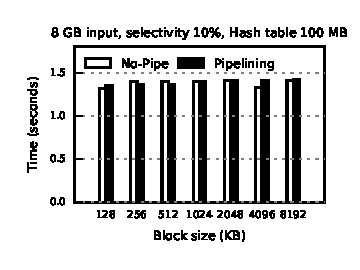
\includegraphics[width=\textwidth]{pipeline/figures/microbenchmark-8gbinput-100mbht-selectivity10pc}	
		\caption{Selectivity 10\%, 100 MB hash table}
	\end{subfigure}
	~
	\begin{subfigure}[ht]{0.32\textwidth}
		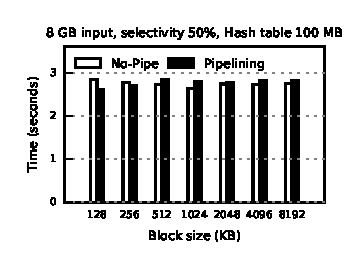
\includegraphics[width=\textwidth]{pipeline/figures/microbenchmark-8gbinput-100mbht-selectivity50pc}	
		\caption{Selectivity 50\%, 100 MB hash table}		
	\end{subfigure}
	~
	\begin{subfigure}[ht]{0.32\textwidth}
		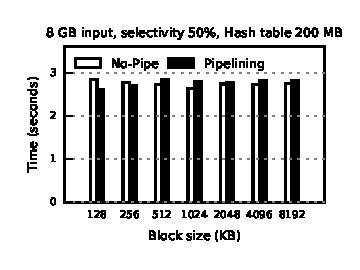
\includegraphics[width=\textwidth]{pipeline/figures/microbenchmark-8gbinput-200mbht-selectivity50pc}	
		\caption{Selectivity 50\%, 200 MB hash table}
	\end{subfigure}
	\caption{\textbf{Results of the micro-benchmarking experiments. The size of the base table is 8 GB. }}
	\label{fig:microbenchmarking-results}
\end{figure*}

The results for our micro-benchmarking study are presented in Figure~\ref{fig:microbenchmarking-results}. 
We use the same setup as described in Section~\ref{ssec:hardware-description} and use 10 threads on a single NUMA socket.

We can observe that the difference between pipelining and non-pipelining is small across all the variations.
Second, for larger block sizes, the two strategies behave quite similarly which is in accordance to our explanation in Section~\ref{ssec:large-blocks-difference}.